%%%%%%%%%%%%%%%%%%%%%%%%%%%%%%%%%%%%%%%%%%%%%%%%%%%
\begin{frame}
  \begin{center}
    {\Large Introduction to PyTorch}
    
\tiny{(Ref: Pytorch Official documentation + few other sources, like Lyman Lin (NTU)))}
  \end{center}
\end{frame}

%%%%%%%%%%%%%%%%%%%%%%%%%%%%%%%%%%%%%%%%%%%%%%%%%%%
\begin{frame}[fragile] \frametitle{What is PyTorch?}
  \begin{center}

{\bf Pytorch is a Python-based scientific computing package that is a replacement for NumPy, and uses the power of Graphics Processing Units. It is also a deep learning research platform that provides maximum flexibility and speed.}

  \end{center}

  {\tiny (Ref: How Pytorch gives the big picture with deep learning - Déborah Mesquita)}
\end{frame}

%%%%%%%%%%%%%%%%%%%%%%%%%%%%%%%%%%%%%%%%%%%%%%%%%%%
\begin{frame}[fragile] \frametitle{What is PyTorch?}
\begin{itemize}
\item Developed by Facebook
\item Torch in Lua but Pytorch in python fully
\item Similar to numpy but leverages GPU
\item Deep Learning Library
\item Dynamic Neural Network
\end{itemize}
\begin{center}
\includegraphics[width=0.8\linewidth,keepaspectratio]{pyt4}
\end{center}
\end{frame}

%%%%%%%%%%%%%%%%%%%%%%%%%%%%%%%%%%%%%%%%%%%%%%%%%%%
\begin{frame}[fragile] \frametitle{Basic Paradigms}


\begin{center}
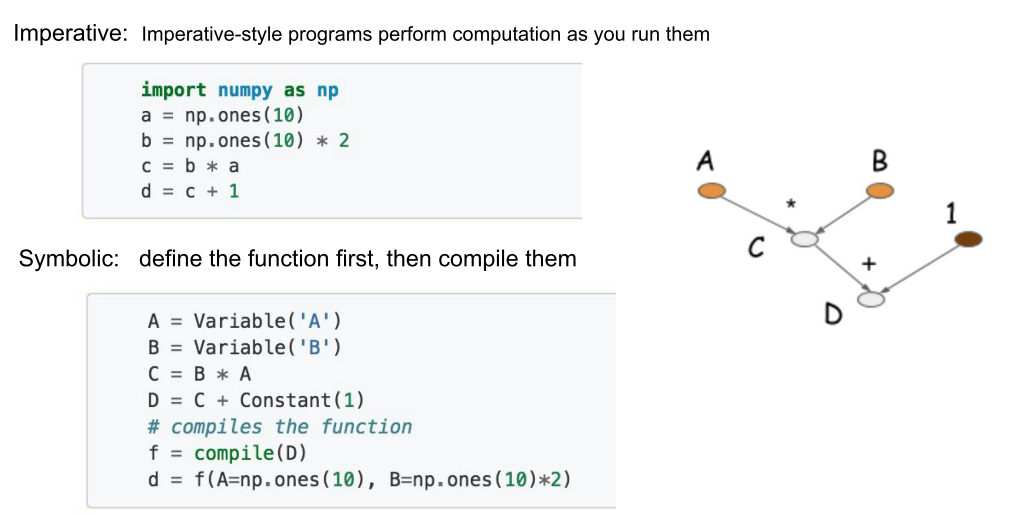
\includegraphics[width=0.9\linewidth,keepaspectratio]{pytorch1}
\end{center}

  {\tiny (Ref: Pytorch Tutorial - Chongruo Wu)}

\end{frame}

%%%%%%%%%%%%%%%%%%%%%%%%%%%%%%%%%%%%%%%%%%%%%%%%%%%
\begin{frame}[fragile] \frametitle{Popular Deep Learning Frameworks}


\begin{center}
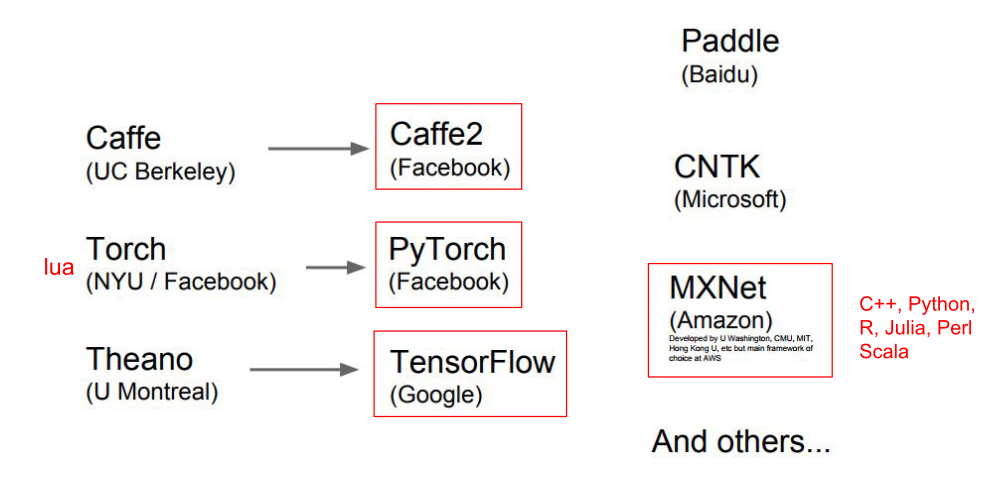
\includegraphics[width=0.9\linewidth,keepaspectratio]{pytorch2}
\end{center}

  {\tiny (Ref: Pytorch Tutorial - Chongruo Wu)}

\end{frame}



%%%%%%%%%%%%%%%%%%%%%%%%%%%%%%%%%%%%%%%%%%%%%%%%%%%
\begin{frame}[fragile] \frametitle{Installation}

Visit https://pytorch.org/get-started/locally/

\begin{center}
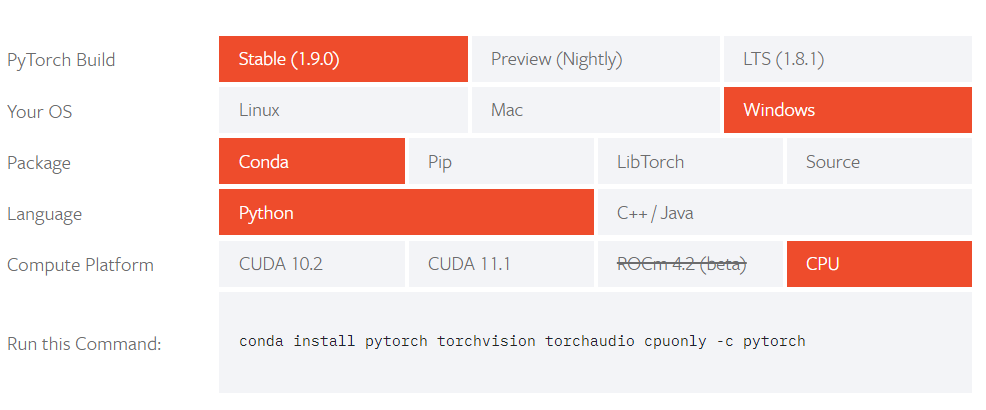
\includegraphics[width=\linewidth,keepaspectratio]{pyt39}%{pyt5}
\end{center}


\end{frame}


%%%%%%%%%%%%%%%%%%%%%%%%%%%%%%%%%%%%%%%%%%%%%%%%%%%
\begin{frame}[fragile] \frametitle{Imp Packages inside PyTorch}
\begin{itemize}
\item  torch: a Tensor library like Numpy, with strong GPU support
\item torch.autograd: an automatic differentiation library 
\item torch.nn: a neural networks library deeply integrated with autograd 
\item torch.optim: an optimization package to be used with torch.nn
\item torch.utils: DataLoader, Trainer and other utility functions for convenience
\end{itemize}
\end{frame}


%%%%%%%%%%%%%%%%%%%%%%%%%%%%%%%%%%%%%%%%%%%%%%%%%%%
\begin{frame}[fragile] \frametitle{Concepts of PyTorch}
\begin{itemize}
\item Data:
\begin{itemize}
\item Tensor
\item Variable (for Gradient)
\end{itemize}
\item Function:
\begin{itemize}
\item   NN Modules
\item   Optimizer
\item   Loss Function
\item   Multi-Processing
\end{itemize}
\end{itemize}
\end{frame}

 % %%%%%%%%%%%%%%%%%%%%%%%%%%%%%%%%%%%%%%%%%%%%%%%%%%%%%%%%%%%%%%%%%%%%%%%%%%%%%%%%%%
\begin{frame}[fragile]
\frametitle{What is a Tensor?}
\begin{itemize}
\item Tensors to encode the inputs and outputs of a model, as well as the model's parameters.
\item Similar to NumPy's ndarrays, except that tensors can run on GPUs or other hardware accelerators. (both actually share same underlying memory, if CPU)

\end{itemize}

 \begin{lstlisting}
import torch
import numpy as np

data = [[1, 2],[3, 4]]
x_data = torch.tensor(data)
x_data_numpy = x_data.numpy()

np_array = np.array(data)
x_np = torch.from_numpy(np_array)

 \end{lstlisting}
 
 
 \end{frame} 
 
 
 % %%%%%%%%%%%%%%%%%%%%%%%%%%%%%%%%%%%%%%%%%%%%%%%%%%%%%%%%%%%%%%%%%%%%%%%%%%%%%%%%%%
\begin{frame}[fragile]
\frametitle{What is a Tensor?}
\begin{itemize}
\item All of deep learning is computations on tensors
\item Array with dimension 0 is a scalar
\item Array with dimension 1 is a vector
\item Array with dimension 2 is a martix
\item Array with dimension 3 or more is a tensor
\item Tensors can be created from Python lists with the torch.tensor() function.
\end{itemize}
 \end{frame} 
 
 % %%%%%%%%%%%%%%%%%%%%%%%%%%%%%%%%%%%%%%%%%%%%%%%%%%%%%%%%%%%%%%%%%%%%%%%%%%%%%%%%%%
\begin{frame}[fragile]
\frametitle{1D Tensor}
1D Vector
 \begin{lstlisting}
 import torch

V_data = [1.,2.,3.]
V = torch.tensor(V_data)
print(V)

>>>tensor([ 1.,  2.,  3.])
 \end{lstlisting}

 \end{frame} 


 
%%%%%%%%%%%%%%%%%%%%%%%%%%%%%%%%%%%%%%%%%%%%%%%%%%%%%%%%%%%%%%%%%%%%%%%%%%%%%%%%%%
\begin{frame}[fragile]
\frametitle{2D Tensor}
Matrix 
 \begin{lstlisting}
M_data = [[1., 2., 3.], [4., 5., 6]]
M = torch.tensor(M_data)
print(M)

>>>tensor([[ 1.,  2.,  3.],
        [ 4.,  5.,  6.]])
 \end{lstlisting}

 \end{frame} 

 
 % %%%%%%%%%%%%%%%%%%%%%%%%%%%%%%%%%%%%%%%%%%%%%%%%%%%%%%%%%%%%%%%%%%%%%%%%%%%%%%%%%%
\begin{frame}[fragile]
\frametitle{3D Tensor}
3D tensor of size 2x2x2.
 \begin{lstlisting}
T_data = [[[1.,2.], [3.,4.]],
          [[5.,6.], [7.,8.]]]
T = torch.tensor(T_data)
print(T)


>>>tensor([[[ 1.,  2.],
         [ 3.,  4.]],

        [[ 5.,  6.],
         [ 7.,  8.]]])
 \end{lstlisting}

 \end{frame} 
 
  % %%%%%%%%%%%%%%%%%%%%%%%%%%%%%%%%%%%%%%%%%%%%%%%%%%%%%%%%%%%%%%%%%%%%%%%%%%%%%%%%%%
\begin{frame}[fragile]
\frametitle{Random, Constant Tensor}

\begin{lstlisting}
shape = (2,3,)
rand_tensor = torch.rand(shape)
ones_tensor = torch.ones(shape)
zeros_tensor = torch.zeros(shape)

print(f"Random Tensor: \n {rand_tensor} \n")
print(f"Ones Tensor: \n {ones_tensor} \n")
print(f"Zeros Tensor: \n {zeros_tensor}")

Random Tensor: 
 tensor([[0.5742, 0.4606, 0.0981],
        [0.3154, 0.0503, 0.0097]]) 

Ones Tensor: 
 tensor([[1., 1., 1.],
        [1., 1., 1.]]) 

Zeros Tensor: 
 tensor([[0., 0., 0.],
        [0., 0., 0.]])
 \end{lstlisting}

 \end{frame} 
 

 % %%%%%%%%%%%%%%%%%%%%%%%%%%%%%%%%%%%%%%%%%%%%%%%%%%%%%%%%%%%%%%%%%%%%%%%%%%%%%%%%%%
\begin{frame}[fragile]
\frametitle{Attributes of Tensor}

\begin{lstlisting}
tensor = torch.rand(3,4)

print(f"Shape of tensor: {tensor.shape}")
print(f"Datatype of tensor: {tensor.dtype}")
print(f"Device tensor is stored on: {tensor.device}")

Shape of tensor: torch.Size([3, 4])
Datatype of tensor: torch.float32
Device tensor is stored on: cpu
 \end{lstlisting}

 \end{frame} 
 
 
 % %%%%%%%%%%%%%%%%%%%%%%%%%%%%%%%%%%%%%%%%%%%%%%%%%%%%%%%%%%%%%%%%%%%%%%%%%%%%%%%%%%
\begin{frame}[fragile]
\frametitle{Indexing}
\begin{itemize}
\item Indexing into the vector gives you a scalar. 
\item Indexing into the matrix gives you a vector. 
\item Indexing into the tensor gives you a matrix!
\end{itemize}

 \begin{lstlisting}
print(V[0])
print(M[0])
print(T[0])

tensor(1.)
tensor([ 1.,  2.,  3.])
tensor([[ 1.,  2.],
        [ 3.,  4.]])
 \end{lstlisting}

 \end{frame} 
 
 
  % %%%%%%%%%%%%%%%%%%%%%%%%%%%%%%%%%%%%%%%%%%%%%%%%%%%%%%%%%%%%%%%%%%%%%%%%%%%%%%%%%%
\begin{frame}[fragile]
\frametitle{Data type}
\begin{itemize}
\item Default datatype in tensor is Float
\item For int tensor, call torch.LongTensor(), etc
\item To create a tensor with random data and the supplied dimensionality with torch.rand()
\end{itemize}

 \end{frame} 
 
%%%%%%%%%%%%%%%%%%%%%%%%%%%%%%%%%%%%%%%%%%%%%%%%%%%%%%%%%%%%%%%%%%%%%%%%%%%%%%%%%%
\begin{frame}[fragile]
\frametitle{Initialization}
 \begin{lstlisting}
x = torch.rand((3, 4, 5))
print(x)

>>>tensor([[[-1.5256, -0.7502, -0.6540, -1.6095, -0.1002],
         [-0.6092, -0.9798, -1.6091, -0.7121,  0.3037],
         [-0.7773, -0.2515, -0.2223,  1.6871,  0.2284],
         [ 0.4676, -0.6970, -1.1608,  0.6995,  0.1991]],

        [[ 0.8657,  0.2444, -0.6629,  0.8073,  1.1017],
         [-0.1759, -2.2456, -1.4465,  0.0612, -0.6177],
         [-0.7981, -0.1316,  1.8793, -0.0721,  0.1578],
         [-0.7735,  0.1991,  0.0457,  0.1530, -0.4757]],

        [[-0.1110,  0.2927, -0.1578, -0.0288,  0.4533],
         [ 1.1422,  0.2486, -1.7754, -0.0255, -1.0233],
         [-0.5962, -1.0055,  0.4285,  1.4761, -1.7869],
         [ 1.6103, -0.7040, -0.1853, -0.9962, -0.8313]]])
 \end{lstlisting}

 \end{frame} 
 
  % %%%%%%%%%%%%%%%%%%%%%%%%%%%%%%%%%%%%%%%%%%%%%%%%%%%%%%%%%%%%%%%%%%%%%%%%%%%%%%%%%%
\begin{frame}[fragile]
\frametitle{Operations on Tensors}
\begin{itemize}
\item 100s of operations available.
\item Each of these operations can be run on the GPU (at typically higher speeds than on a CPU).
\item By default, tensors are created on the CPU. 
\item Need to explicitly move tensors to the GPU using $.to$ method (after checking for GPU availability). 
\item Keep in mind that copying large tensors across devices can be expensive in terms of time and memory!
\end{itemize}

 \begin{lstlisting}
# We move our tensor to the GPU if available
if torch.cuda.is_available():
  tensor = tensor.to('cuda')
 \end{lstlisting}

 \end{frame} 
 
 
 
 %%%%%%%%%%%%%%%%%%%%%%%%%%%%%%%%%%%%%%%%%%%%%%%%%%%%%%%%%%%%%%%%%%%%%%%%%%%%%%%%%%
\begin{frame}[fragile]
\frametitle{Operations}
Operations with Tensors.

 Note:  In-place operations save some memory, but can be problematic when computing derivatives because of an immediate loss of history. Hence, their use is discouraged.
 
 
 \begin{lstlisting}
x = torch.tensor([1.,2.,3.])
y = torch.tensor([4.,5.,6.])
z = x + y
print(z)

>>>tensor([ 5.,  7.,  9.])

# Operations that store the result into the operand are called in-place. They are denoted by a _ suffix. For example: x.copy_(y), x.t_(), will change x.
 
tensor.add_(5)
\end{lstlisting}

\end{frame} 
 
 %%%%%%%%%%%%%%%%%%%%%%%%%%%%%%%%%%%%%%%%%%%%%%%%%%%%%%%%%%%%%%%%%%%%%%%%%%%%%%%%%%
\begin{frame}[fragile]
\frametitle{Operations}
Multiplication:

Many more mathematical operations are available.

\begin{lstlisting}
# This computes the matrix multiplication between two tensors. y1, y2, y3 will have the same value
y1 = tensor @ tensor.T
y2 = tensor.matmul(tensor.T)

y3 = torch.rand_like(tensor)
torch.matmul(tensor, tensor.T, out=y3)


# This computes the element-wise product. z1, z2, z3 will have the same value
z1 = tensor * tensor
z2 = tensor.mul(tensor)

z3 = torch.rand_like(tensor)
torch.mul(tensor, tensor, out=z3)
\end{lstlisting}
\end{frame} 
 
 
%%%%%%%%%%%%%%%%%%%%%%%%%%%%%%%%%%%%%%%%%%%%%%%%%%%%%%%%%%%%%%%%%%%%%%%%%%%%%%%%%%
\begin{frame}[fragile]
\frametitle{Concatenation}
Concatenation
 \begin{lstlisting}
# By default, it concatenates along the first axis (concatenates rows)
x_1 = torch.randn(2, 5)
y_1 = torch.randn(3, 5)
z_1 =torch.cat([x_1, y_1])
print(z_1)

# Concatenate columns:
x_2 = torch.randn(2, 3)
y_2 = torch.randn(2, 5)
z_2 = torch.cat([x_2, y_2], 1) # second arg specifies which axis to concat along
print(z_2)

# If your tensors are not compatible, torch will complain.  Uncomment to see the error
# torch.cat([x_1, x_2])
\end{lstlisting}
\end{frame} 
 
 %%%%%%%%%%%%%%%%%%%%%%%%%%%%%%%%%%%%%%%%%%%%%%%%%%%%%%%%%%%%%%%%%%%%%%%%%%%%%%%%%%
\begin{frame}[fragile]
\frametitle{Reshaping}
Reshaping Tensors with view() method.

If one of the dimensions is -1, its size can be inferred

\begin{lstlisting}
x = torch.randn(2,3,4)
print(x)
print(x.view(2,12)) # Reshape to 2 rows, 12 columns
print(x.view(2, -1)) # Same as above. 
\end{lstlisting}
\end{frame} 
 
%%%%%%%%%%%%%%%%%%%%%%%%%%%%%%%%%%%%%%%%%%%%%%%%%%%%%%%%%%%%%%%%%%%%%%%%%%%%%%%%%%
\begin{frame}[fragile]
\frametitle{Computation Graphs}

\begin{itemize}
\item It is a specification of how your data is combined to give you the output. 
\item Since the graph totally specifies what parameters were involved with which operations, it contains enough information to compute derivatives.
\end{itemize}
\end{frame} 

 
 %%%%%%%%%%%%%%%%%%%%%%%%%%%%%%%%%%%%%%%%%%%%%%%%%%%%%%%%%%%%%%%%%%%%%%%%%%%%%%%%%%
\begin{frame}[fragile]
\frametitle{Variables and Tensors}
\begin{itemize}
\item What does torch.tensor object has stored? : data and the shape, and maybe a few other things
\item But when we added two tensors together, we got an output tensor. 
\item All this output tensor knows is its data and shape. 
\item It has no idea that it was the sum of two other tensors (it could have been read in from a file, it could be the result of some other operation, etc.)
\item The Variable class keeps track of how it was created. 
\end{itemize}
Latest News: Variables and Tensors have merged!!!
\end{frame} 
 
 
%%%%%%%%%%%%%%%%%%%%%%%%%%%%%%%%%%%%%%%%%%%%%%%%%%%%%%%%%%%%%%%%%%%%%%%%%%%%%%%%%%
\begin{frame}[fragile]
\frametitle{PyTorch 0.4.0 release notes}
\begin{itemize}
\item Tensors and Variables have merged
\item torch.autograd.Variable and torch.tensor are now the same class. 
\item More precisely, torch.tensor is capable of tracking history and behaves like the old Variable; Variable wrapping continues to work as before but returns an object of type torch.tensor. \item No need the Variable wrapper everywhere in your code anymore.
\end{itemize}
 \begin{lstlisting}
>>> x = torch.DoubleTensor([1, 1, 1])
>>> print(type(x)) # was torch.DoubleTensor
<class 'torch.autograd.variable.Variable'>
>>> print(x.type())  # OK: 'torch.DoubleTensor'
'torch.DoubleTensor'
>>> print(isinstance(x, torch.DoubleTensor))  # OK: True
True
\end{lstlisting}
\end{frame} 
 
    %%%%%%%%%%%%%%%%%%%%%%%%%%%%%%%%%%%%%%%%%%%%%%%%%%%%%%%%%%%%%%%%%%%%%%%%%%%%%%%%%%
\begin{frame}[fragile]
\frametitle{PyTorch 0.4.0 release notes}

\begin{itemize}
\item When does autograd start tracking history now?
\item requires\_grad, the central flag for autograd, is now an attribute on Tensors.
\end{itemize}
 \begin{lstlisting}
>>> x = torch.ones(1)  # create a tensor with requires_grad=False (default)
>>> x.requires_grad
False
>>> y = torch.ones(1)  # another tensor with requires_grad=False
>>> z = x + y
>>> # both inputs have requires_grad=False. so does the output
>>> z.requires_grad
False
>>> # then autograd won't track this computation. let's verify!
>>> z.backward()
RuntimeError: element 0 of tensors does not require grad and does not have a grad_fn
\end{lstlisting}
\end{frame} 
 
     %%%%%%%%%%%%%%%%%%%%%%%%%%%%%%%%%%%%%%%%%%%%%%%%%%%%%%%%%%%%%%%%%%%%%%%%%%%%%%%%%%
\begin{frame}[fragile]
\frametitle{PyTorch 0.4.0 release notes}

 \begin{lstlisting}
>>>
>>> # now create a tensor with requires_grad=True
>>> w = torch.ones(1, requires_grad=True)
>>> w.requires_grad
True
>>> # add to the previous result that has require_grad=False
>>> total = w + z
>>> # the total sum now requires grad!
>>> total.requires_grad
True
>>> # autograd can compute the gradients as well
>>> total.backward()
>>> w.grad
tensor([ 1.])
>>> # and no computation is wasted to compute gradients for x, y and z, which don't require grad
>>> z.grad == x.grad == y.grad == None
True
\end{lstlisting}
\end{frame} 
 
     %%%%%%%%%%%%%%%%%%%%%%%%%%%%%%%%%%%%%%%%%%%%%%%%%%%%%%%%%%%%%%%%%%%%%%%%%%%%%%%%%%
\begin{frame}[fragile]
\frametitle{PyTorch 0.4.0 release notes}

\begin{itemize}
\item What about .data?
\item .data was the primary way to get the underlying Tensor from a Variable. 
\item After this merge, calling y = x.data still has similar semantics.
\item So y will be a Tensor that shares the same data with x, is unrelated with the computation history of x, and has requires\_grad=False.
\end{itemize}

From now onwards, even if Variables and Tensors are mentioned disticnlty, from 0.4.0, they are just the Tensors with grad\_fn available.
\end{frame} 
 
 
  
  %%%%%%%%%%%%%%%%%%%%%%%%%%%%%%%%%%%%%%%%%%%%%%%%%%%%%%%%%%%%%%%%%%%%%%%%%%%%%%%%%%
\begin{frame}[fragile]
\frametitle{Tensor/Variables operations}

So now, what is the derivative of this sum with respect to the first component of x? 


 \begin{lstlisting}
x = torch.tensor([1.,2.,3.])
y = torch.tensor([4.,5.,6.])
x.requires_grad = True
y.requires_grad = True
z = x + y
print(z.data)
>>>tensor([ 5.,  7.,  9.])
print(z.grad_fn)
>>><AddBackward1 object at 0x000000000A9C94A8>
s = z.sum()
print(s.data)
>>>tensor(21.)
print(s.grad_fn)
>>><SumBackward0 object at 0x000000000A9C94E0>
\end{lstlisting}
\end{frame} 
 
%%%%%%%%%%%%%%%%%%%%%%%%%%%%%%%%%%%%%%%%%%%%%%%%%%%%%%%%%%%%%%%%%%%%%%%%%%%%%%%%%%
\begin{frame}[fragile]
\frametitle{Derivative}
\begin{itemize}
\item Need $\frac{\partial s}{\partial x_0}$
\item s knows that it was created as a sum of the tensor z. 
\item z knows that it was the sum x + y. 
\item So, $s = \overbrace{x_0 + y_0}^\text{$z_0$} + \overbrace{x_1 + y_1}^\text{$z_1$} + \overbrace{x_2 + y_2}^\text{$z_2$}$
\item Enough information to determine that the derivative : Pytorch knows how to compute their gradients of sum() and + operations, and run the back propagation algorithm. 
\end{itemize}


\end{frame} 
 
 %%%%%%%%%%%%%%%%%%%%%%%%%%%%%%%%%%%%%%%%%%%%%%%%%%%%%%%%%%%%%%%%%%%%%%%%%%%%%%%%%%
\begin{frame}[fragile]
\frametitle{Back Propagation}

\begin{lstlisting}
s.backward() # calling .backward() on any variable will run backprop, starting from it.
print(x.grad)

>>>tensor([ 1.,  1.,  1.])
\end{lstlisting}

\end{frame} 
 
 
  %%%%%%%%%%%%%%%%%%%%%%%%%%%%%%%%%%%%%%%%%%%%%%%%%%%%%%%%%%%%%%%%%%%%%%%%%%%%%%%%%%
\begin{frame}[fragile]
\frametitle{Variable Gradient}
Note:
 \begin{lstlisting}
x = torch.randn((2,2))
y = torch.randn((2,2))
x.requires_grad = True
y.requires_grad = True
z = x + y 
print(z.grad_fn)
>>><AddBackward1 object at 0x000000000A9D2358>

var_z_data = z.data # Get the wrapped Tensor object out of var_z...
new_var_z = torch.tensor( var_z_data ) # Re-wrap the tensor in a new variable

# does new_var_z have info to backprop to x and y? NO!
print(new_var_z.grad_fn)
>>>None
# And how could it?  We copied the tensor values out of z (that is what z.data is).  This tensor doesn't know anything about how it was computed.   If var_z_data doesn't know how it was computed, theres no way new_var_z will.
\end{lstlisting}

\end{frame} 
 

%%%%%%%%%%%%%%%%%%%%%%%%%%%%%%%%%%%%%%%%%%%%%%%%%%%
\begin{frame}[fragile] \frametitle{Autograd: automatic gradient}
\begin{itemize}
\item Provides automatic differentiation for all operations on Tensors
\item It is a define-by-run framework, which means that your backprop is defined by how your code is run, and that every single iteration can be different.
\end{itemize}
\end{frame}

%%%%%%%%%%%%%%%%%%%%%%%%%%%%%%%%%%%%%%%%%%%%%%%%%%%
\begin{frame}[fragile] \frametitle{Automatic differentiation}

\begin{itemize}
\item In $backpropogation$ parameters (model weights) are adjusted according to the gradient of the loss function with respect to the given parameter.
\item To compute those gradients, PyTorch has a built-in differentiation engine called \lstinline|torch.autograd|. 
\item It supports automatic computation of gradient for any computational graph.
\item Consider the simplest one-layer neural network, with input x, parameters w and b, and some loss function.
\end{itemize}

\tiny{(Ref: Microsoft - Intro to Machine Learning using Pytorch)}


\begin{lstlisting}
import torch

x = torch.ones(5)  # input tensor
y = torch.zeros(3)  # expected output
w = torch.randn(5, 3, requires_grad=True)
b = torch.randn(3, requires_grad=True)
z = torch.matmul(x, w)+b
loss = torch.nn.functional.binary_cross_entropy_with_logits(z, y)
\end{lstlisting}

\end{frame}

%%%%%%%%%%%%%%%%%%%%%%%%%%%%%%%%%%%%%%%%%%%%%%%%%%%
\begin{frame}[fragile] \frametitle{Tensors, Functions and Computational graph}

\begin{center}
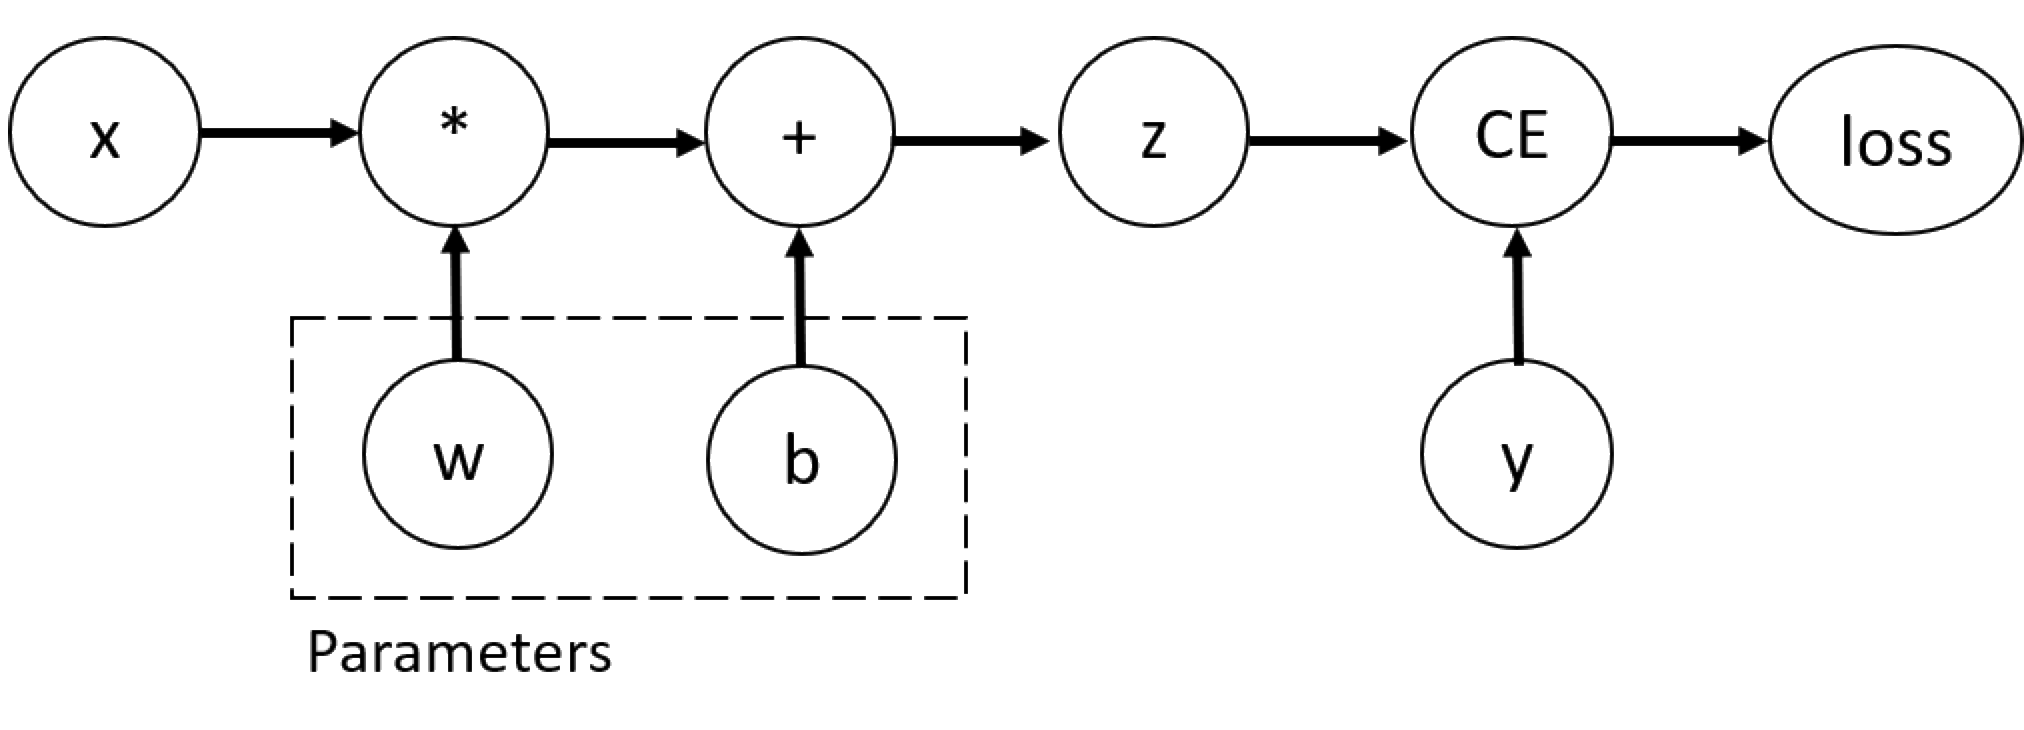
\includegraphics[width=\linewidth,keepaspectratio]{pyt40}
\end{center}

\begin{itemize}
\item In this network, w and b are parameters, which need to be optimized. 
\item Need to be able to compute the gradients of loss function with respect to those variables. 
\item Set the \lstinline|requires_grad| property of those tensors. Note: You can set the value of \lstinline|requires_grad| when creating a tensor, or later by using \lstinline|x.requires_grad_(True)| method.
\end{itemize}


\tiny{(Ref: Microsoft - Intro to Machine Learning using Pytorch)}
\end{frame}

%%%%%%%%%%%%%%%%%%%%%%%%%%%%%%%%%%%%%%%%%%%%%%%%%%%
\begin{frame}[fragile] \frametitle{Tensors, Functions and Computational graph}


\begin{itemize}
\item A function that we apply to tensors to construct computational graph is in fact an object of class Function. 
\item This object knows how to compute the function in the forward direction, and also how to compute its derivative during the backward propagation step. 
\item A reference to the backward propagation function is stored in \lstinline|grad_fn| property of a tensor.
\end{itemize}

\tiny{(Ref: Microsoft - Intro to Machine Learning using Pytorch)}


\begin{lstlisting}
print('Gradient function for z =',z.grad_fn)
print('Gradient function for loss =', loss.grad_fn)

>>>Gradient function for z = <AddBackward0 object at 0x7fcaa4928110>
Gradient function for loss = <BinaryCrossEntropyWithLogitsBackward object at 0x7fcaa4928250>
\end{lstlisting}

\end{frame}

%%%%%%%%%%%%%%%%%%%%%%%%%%%%%%%%%%%%%%%%%%%%%%%%%%%
\begin{frame}[fragile] \frametitle{Computing gradients}

\begin{itemize}
\item To optimize weights of parameters in the neural network, we need to compute the derivatives of our loss function with respect to parameters, namely, we need  $\frac{\partial loss}{\partial w}$ and
$\frac{\partial loss}{\partial b}$   under some fixed values of x and y. 
\item To compute those derivatives, we call \lstinline|loss.backward()|, and then retrieve the values from \lstinline|w.grad| and \lstinline|b.grad|:
\end{itemize}

\tiny{(Ref: Microsoft - Intro to Machine Learning using Pytorch)}


\begin{lstlisting}
loss.backward()
print(w.grad)
print(b.grad)

>>>tensor([[0.2739, 0.0490, 0.3279],
        [0.2739, 0.0490, 0.3279],
        [0.2739, 0.0490, 0.3279],
        [0.2739, 0.0490, 0.3279],
        [0.2739, 0.0490, 0.3279]])
tensor([0.2739, 0.0490, 0.3279])
\end{lstlisting}

\end{frame}

%%%%%%%%%%%%%%%%%%%%%%%%%%%%%%%%%%%%%%%%%%%%%%%%%%%
\begin{frame}[fragile] \frametitle{Computing gradients}

Note:
\begin{itemize}
\item We can only obtain the grad properties for the leaf nodes of the computational graph, which have \lstinline|requires_grad| property set to True. 
\item For all other nodes in our graph, gradients will not be available. 
\item In addition, we can only perform gradient calculations using backward once on a given graph, for performance reasons. 
\item If we need to do several backward calls on the same graph, we need to pass \lstinline|retain_graph=True| to the backward call.
\item By default, all tensors with \lstinline|requires_grad=True| are tracking their computational history and support gradient computation. 
\item However, if we only want to do forward computations through the network. We can stop tracking computations by surrounding our computation code with \lstinline|torch.no_grad()| block.
\item Disabling can also be used to mark some parameters in your neural network at frozen parameters, say, for pre-trained networks.
\end{itemize}

\tiny{(Ref: Microsoft - Intro to Machine Learning using Pytorch)}



\end{frame}

%%%%%%%%%%%%%%%%%%%%%%%%%%%%%%%%%%%%%%%%%%%%%%%%%%%
\begin{frame}[fragile] \frametitle{Computing gradients}

\tiny{(Ref: Microsoft - Intro to Machine Learning using Pytorch)}


\begin{lstlisting}
z = torch.matmul(x, w)+b
print(z.requires_grad)

with torch.no_grad():
    z = torch.matmul(x, w)+b
print(z.requires_grad)

>>>True
False
\end{lstlisting}

\end{frame}


%%%%%%%%%%%%%%%%%%%%%%%%%%%%%%%%%%%%%%%%%%%%%%%%%%%
\begin{frame}[fragile] \frametitle{Computational Graphs}


\begin{itemize}
\item Conceptually, autograd keeps a record of data (tensors) and all executed operations (along with the resulting new tensors) in a directed acyclic graph (DAG) consisting of Function objects. 
\item In this DAG, leaves are the input tensors, roots are the output tensors. 
\item By tracing this graph from roots to leaves, you can automatically compute the gradients using the chain rule.
\item In a forward pass, autograd does two things simultaneously:
	\begin{itemize}
	\item run the requested operation to compute a resulting tensor
	\item maintain the operation’s gradient function in the DAG.
	\end{itemize}
\item The backward pass kicks off when .backward() is called on the DAG root. autograd then:
	\begin{itemize}
	\item computes the gradients from each \lstinline|.grad_fn|,
	\item accumulates them in the respective tensor’s \lstinline|.grad| attribute
	\item using the chain rule, propagates all the way to the leaf tensors.
	\end{itemize}

\end{itemize}


\tiny{(Ref: Microsoft - Intro to Machine Learning using Pytorch)}
\end{frame}

%%%%%%%%%%%%%%%%%%%%%%%%%%%%%%%%%%%%%%%%%%%%%%%%%%%
\begin{frame}[fragile] \frametitle{Computional Graphs}
DAGs are dynamic in PyTorch

\begin{itemize}
\item The graph is recreated from scratch; after each \lstinline|.backward()| call, autograd starts populating a new graph. 
\item This is exactly what allows you to use control flow statements in your model; you can change the shape, size and operations at every iteration if needed.
\end{itemize}


\tiny{(Ref: Microsoft - Intro to Machine Learning using Pytorch)}
\end{frame}

%%%%%%%%%%%%%%%%%%%%%%%%%%%%%%%%%%%%%%%%%%%%%%%%%%%
\begin{frame}[fragile] \frametitle{Computional Graphs}
Odd cases
\begin{itemize}
\item In case of a scalar loss function, and we need to compute the gradient with respect to some parameters. 
\item However, there are cases when the output function is an arbitrary tensor. 
\item In this case, PyTorch allows you to compute so-called Jacobian product, and not the actual gradient.
\item For a vector function $\vec{y}=f(\vec{x})$, where
$\vec{x}=\langle x_1,\dots,x_n\rangle$ and
$\vec{y}=\langle y_1,\dots,y_m\rangle$, a gradient of
$\vec{y}$ with respect to $\vec{x}$ is given by \lstinline|Jacobian matrix|

% \begin{align}
% \begin{align}J=\left(\begin{array}{ccc}
      % \frac{\partial y_{1}}{\partial x_{1}} & \cdots & \frac{\partial y_{1}}{\partial x_{n}}\\
      % \vdots & \ddots & \vdots\\
      % \frac{\partial y_{m}}{\partial x_{1}} & \cdots & \frac{\partial y_{m}}{\partial x_{n}}
      % \end{array}\right)
% \end{align}
% \end{align}

\item Instead of computing the Jacobian matrix itself, PyTorch allows you to
compute **Jacobian Product** $v^T\cdot J$ for a given input vector
$v=(v_1 \dots v_m)$. This is achieved by calling `backward` with
$v$ as an argument. The size of $v$ should be the same as
the size of the original tensor, with respect to which we want to
compute the product
\end{itemize}


\tiny{(Ref: Microsoft - Intro to Machine Learning using Pytorch)}
\end{frame}


%%%%%%%%%%%%%%%%%%%%%%%%%%%%%%%%%%%%%%%%%%%%%%%%%%%
\begin{frame}[fragile] \frametitle{Computational Graphs}

\begin{itemize}
\item Notice that when we call backward for the second time with the same argument, the value of the gradient is different. 
\item This happens because PyTorch accumulates the gradients, i.e. the value of computed gradients is added to the grad property of all leaf nodes of computational graph. 
\item If you want to compute the proper gradients, you need to zero out the grad property before. 
\item \lstinline|backward()| is equivalent to calling \lstinline|backward(torch.tensor(1.0))|, which is a useful way to compute the gradients in case of a scalar-valued function, such as loss during neural network training.
\end{itemize}


\tiny{(Ref: Microsoft - Intro to Machine Learning using Pytorch)}




\end{frame}

%%%%%%%%%%%%%%%%%%%%%%%%%%%%%%%%%%%%%%%%%%%%%%%%%%%
\begin{frame}[fragile] \frametitle{Computational Graphs}


\tiny{(Ref: Microsoft - Intro to Machine Learning using Pytorch)}

\begin{lstlisting}
inp = torch.eye(5, requires_grad=True)
out = (inp+1).pow(2)
out.backward(torch.ones_like(inp), retain_graph=True)
print("First call\n", inp.grad)
out.backward(torch.ones_like(inp), retain_graph=True)
print("\nSecond call\n", inp.grad)
inp.grad.zero_()
out.backward(torch.ones_like(inp), retain_graph=True)
print("\nCall after zeroing gradients\n", inp.grad)

\end{lstlisting}


\end{frame}

% %%%%%%%%%%%%%%%%%%%%%%%%%%%%%%%%%%%%%%%%%%%%%%%%%%%
% \begin{frame}[fragile] \frametitle{Function}
% \begin{itemize}
% \item Implements forward and backward definitions of an autograd operation. 
% \item Every Variable operation, creates at least a single Function node, that connects to functions that created a Variable and encodes its history.
% \item Variable and Function are interconnected and build up an acyclic graph, that encodes a complete history of computation.
% \item Each variable has a .grad\_fn attribute that references a Function that has created the Variable (except for Variables created by the user - their grad\_fn is None).
% \end{itemize}
% \end{frame}

%%%%%%%%%%%%%%%%%%%%%%%%%%%%%%%%%%%%%%%%%%%%%%%%%%%%%%%%%%%%%%%%%%%%%%%%%%%%%%%%%%
\begin{frame}[fragile]
\frametitle{Activation Functions}

\begin{itemize}
\item Neural network consists of composing linearities with non-linearities, a long chains of affine compositions.
\item Non-linearities like $\tanh(x), \sigma(x), \text{ReLU}(x)$ are the most common.
\item Why these functions? I can think of plenty of other non-linearities.
\end{itemize}
\end{frame} 

%%%%%%%%%%%%%%%%%%%%%%%%%%%%%%%%%%%%%%%%%%%%%%%%%%%%%%%%%%%%%%%%%%%%%%%%%%%%%%%%%%
\begin{frame}[fragile]
\frametitle{Activation}

\begin{itemize}
\item The reason for this is that they have gradients that are easy to compute, and computing gradients is essential for learning. For example $ \frac{d\sigma}{dx} = \sigma(x)(1 - \sigma(x)) $
\item $ \sigma(x)$ less popular because the gradient vanishes very quickly as the absolute value of the argument grows. Small gradients means it is hard to learn. Most use tanh or ReLU.
\end{itemize}

 Note, all negatives are made 0 and positives kept as they are.

\begin{lstlisting}
data = torch.randn(2,2,requires_grad=True)
print(data)
import torch.nn.functional as F
print(F.relu(data))
>>>tensor([[ 1.6169, -0.9026],
			[ 0.1737,  0.0772]])
tensor([[ 1.6169,  0.0000],
			[ 0.1737,  0.0772]])
\end{lstlisting}
\end{frame} 

%%%%%%%%%%%%%%%%%%%%%%%%%%%%%%%%%%%%%%%%%%%%%%%%%%%%%%%%%%%%%%%%%%%%%%%%%%%%%%%%%%
\begin{frame}[fragile]
\frametitle{Softmax and Probabilities}

It should be clear that the output is a probability distribution: each element is non-negative and the sum over all components is 1.

\begin{itemize}
\item The function $\text{Softmax}(x)$ is also just a non-linearity, but it is special in that it usually is the last operation done in a network. 
\item This is because it takes in a vector of real numbers and returns a probability distribution.
\end{itemize}
 \begin{lstlisting}
data = torch.randn(5,requires_grad=True)
print(data)
print(F.softmax(data,0))
print(F.softmax(data,0).sum())

>>>tensor([ 0.1896, -0.2204,  0.1491,  0.0100, -0.1243])
tensor([ 0.2387,  0.1584,  0.2292,  0.1994,  0.1744])
tensor(1.)
 \end{lstlisting}

\end{frame} 

%%%%%%%%%%%%%%%%%%%%%%%%%%%%%%%%%%%%%%%%%%%%%%%%%%%%%%%%%%%%%%%%%%%%%%%%%%%%%%%%%%
\begin{frame}[fragile]
\frametitle{Objective or Loss or Cost function}

\begin{itemize}
\item Neural network is being trained to minimize it.
\item The parameters of the model are then updated by taking the derivative of the loss function. 
\item An example loss function is the negative log likelihood loss, which is a very common objective for multi-class classification.
\item We can compute gradients with respect to all of the parameters used to compute it! Then we can perform standard gradient updates.
\item Let $\theta$ be our parameters,  $L(\theta)$ the loss function, and $\eta$ a positive learning rate. Then:

$$ \theta^{(t+1)} = \theta^{(t)} - \eta \nabla_\theta L(\theta) $$
\end{itemize}

\end{frame} 

%%%%%%%%%%%%%%%%%%%%%%%%%%%%%%%%%%%%%%%%%%%%%%%%%%%%%%%%%%%%%%%%%%%%%%%%%%%%%%%%%%
\begin{frame}[fragile]
\frametitle{Optimization}

\begin{itemize}
\item Training a model is an iterative process; in each iteration (called an epoch) the model makes a guess about the output, calculates the error in its guess (loss), collects the derivatives of the error with respect to its parameters (as we saw in the module), and optimizes these parameters using gradient descent.
\item Many optimization methods do something more than just this vanilla gradient update.
\item Many attempt to vary the learning rate based on what is happening at train time. 
\item Torch provies many in the torch.optim package, and they are all completely transparent. 
\item Using the simplest gradient update is the same as the more complicated algorithms. 
\item Trying different algorithms and different parameters 
\item Other choices: Adam or RMSProp will boost performance noticably.
\end{itemize}

\end{frame} 

%%%%%%%%%%%%%%%%%%%%%%%%%%%%%%%%%%%%%%%%%%%%%%%%%%%
\begin{frame}[fragile] \frametitle{Setting hyperparameters}

Hyperparameters are adjustable parameters that let you control the model optimization process. Example:

\begin{itemize}
\item Number of Epochs: the number times to iterate over the dataset
\item Batch Size: the number of data samples seen by the model in each epoch
\item Learning Rate : how much to update models parameters at each batch/epoch. Smaller values yield slow learning speed, while large values may result in unpredictable behavior during training.
\end{itemize}




Each epoch consists of two main parts:

\begin{itemize}
\item The Train Loop: iterate over the training dataset and try to converge to optimal parameters.
\item The Validation/Test Loop: iterate over the test dataset to check if model performance is improving.
\end{itemize}

\tiny{(Ref: Microsoft - Intro to Machine Learning using Pytorch)}

\begin{lstlisting}
learning_rate = 1e-3
batch_size = 64
epochs = 5
\end{lstlisting}
\end{frame}


%%%%%%%%%%%%%%%%%%%%%%%%%%%%%%%%%%%%%%%%%%%%%%%%%%%
\begin{frame}[fragile] \frametitle{Loss}


\begin{itemize}
\item Loss function measures the degree of dissimilarity of obtained result to the target value, and it is the loss function that we want to minimize during training. \item To calculate the loss we make a prediction using the inputs of our given data sample and compare it against the true data label value.
\item Common loss functions include \lstinline|nn.MSELoss| (Mean Square Error) for regression tasks, and \lstinline|nn.NLLLoss| (Negative Log Likelihood) for classification. 
\item \lstinline|nn.CrossEntropyLoss| combines \lstinline|nn.LogSoftmax| and \lstinline|nn.NLLLoss|.
\end{itemize}

\tiny{(Ref: Microsoft - Intro to Machine Learning using Pytorch)}

\begin{lstlisting}
# Initialize the loss function
loss_fn = nn.CrossEntropyLoss()
\end{lstlisting}

\end{frame}

%%%%%%%%%%%%%%%%%%%%%%%%%%%%%%%%%%%%%%%%%%%%%%%%%%%
\begin{frame}[fragile] \frametitle{Optimization pass}


\begin{itemize}
\item Optimization is the process of adjusting model parameters to reduce model error in each training step. 
\item Optimization algorithms define how this process is performed (in this example we use Stochastic Gradient Descent). 
\item All optimization logic is encapsulated in the optimizer object. Here, we use the SGD optimizer; additionally, there are many different optimizers available in PyTorch such as ADAM and RMSProp, that work better for different kinds of models and data.
\item We initialize the optimizer by registering the model's parameters that need to be trained, and passing in the learning rate hyperparameter.
\end{itemize}

\tiny{(Ref: Microsoft - Intro to Machine Learning using Pytorch)}


\begin{lstlisting}
optimizer = torch.optim.SGD(model.parameters(), lr=learning_rate)
\end{lstlisting}

\end{frame}

%%%%%%%%%%%%%%%%%%%%%%%%%%%%%%%%%%%%%%%%%%%%%%%%%%%
\begin{frame}[fragile] \frametitle{Optimization Pass}

Inside the training loop, optimization happens in three steps:

\begin{itemize}
\item Call \lstinline|optimizer.zero_grad()| to reset the gradients of model parameters. Gradients by default add up; to prevent double-counting, we explicitly zero them at each iteration.
\item Back-propagate the prediction loss with a call to \lstinline|loss.backwards()|. PyTorch deposits the gradients of the loss w.r.t. each parameter.
\item Once we have our gradients, we call \lstinline|optimizer.step()| to adjust the parameters by the gradients collected in the backward pass.
\item We initialize the loss function and optimizer, and pass it to \lstinline|train_loop| and \lstinline|test_loop|.
\end{itemize}


\tiny{(Ref: Microsoft - Intro to Machine Learning using Pytorch)}
\end{frame}

%%%%%%%%%%%%%%%%%%%%%%%%%%%%%%%%%%%%%%%%%%%%%%%%%%%
\begin{frame}[fragile] \frametitle{Training Loop}

\tiny{(Ref: Microsoft - Intro to Machine Learning using Pytorch)}

\begin{lstlisting}
def train_loop(dataloader, model, loss_fn, optimizer):
    size = len(dataloader.dataset)
    for batch, (X, y) in enumerate(dataloader):        
        # Compute prediction and loss
        pred = model(X)
        loss = loss_fn(pred, y)
        
        # Backpropagation
        optimizer.zero_grad()
        loss.backward()
        optimizer.step()

        if batch % 100 == 0:
            loss, current = loss.item(), batch * len(X)
            print(f"loss: {loss:>7f}  [{current:>5d}/{size:>5d}]")
\end{lstlisting}

\end{frame}




%%%%%%%%%%%%%%%%%%%%%%%%%%%%%%%%%%%%%%%%%%%%%%%%%%%
\begin{frame}[fragile] \frametitle{Testing Loop}

\tiny{(Ref: Microsoft - Intro to Machine Learning using Pytorch)}

\begin{lstlisting}
def test_loop(dataloader, model, loss_fn):
    size = len(dataloader.dataset)
    test_loss, correct = 0, 0

    with torch.no_grad():
        for X, y in dataloader:
            pred = model(X)
            test_loss += loss_fn(pred, y).item()
            correct += (pred.argmax(1) == y).type(torch.float).sum().item()
            
    test_loss /= size
    correct /= size
    print(f"Test Error: \n Accuracy: {(100*correct):>0.1f}%, Avg loss: {test_loss:>8f} \n")
\end{lstlisting}

\end{frame}


%%%%%%%%%%%%%%%%%%%%%%%%%%%%%%%%%%%%%%%%%%%%%%%%%%%
\begin{frame}[fragile] \frametitle{Iterations}

\tiny{(Ref: Microsoft - Intro to Machine Learning using Pytorch)}


\begin{lstlisting}
loss_fn = nn.CrossEntropyLoss()
optimizer = torch.optim.SGD(model.parameters(), lr=learning_rate)

epochs = 10
for t in range(epochs):
    print(f"Epoch {t+1}\n-------------------------------")
    train_loop(train_dataloader, model, loss_fn, optimizer)
    test_loop(test_dataloader, model, loss_fn)
print("Done!")
\end{lstlisting}

\end{frame}



%%%%%%%%%%%%%%%%%%%%%%%%%%%%%%%%%%%%%%%%%%%%%%%%%%%
\begin{frame}[fragile] \frametitle{Save and load the model}

\lstinline|torch.save| persists \lstinline|state_dict| which is an internal state dictionary storing the learned parameters.

Note: Be sure to call model.eval() method before inferencing to set the dropout and batch normalization layers to evaluation mode. Failing to do this will yield inconsistent inference results.

\tiny{(Ref: Microsoft - Intro to Machine Learning using Pytorch)}

\begin{lstlisting}
model = models.vgg16(pretrained=True)
torch.save(model.state_dict(), 'data/model_weights.pth')

# load_state_dict() load the parameters 

model = models.vgg16() # we do not specify pretrained=True, i.e. do not load default weights
model.load_state_dict(torch.load('data/model_weights.pth'))
model.eval()
\end{lstlisting}


\end{frame}


%%%%%%%%%%%%%%%%%%%%%%%%%%%%%%%%%%%%%%%%%%%%%%%%%%%
\begin{frame}[fragile] \frametitle{Save and load the model}

If we want to store the architecture also, along with weights then pass the whole model to \lstinline|torch.save|

Note: This approach uses Python pickle module when serializing the model, thus it relies on the actual class definition to be available when loading the model.

\tiny{(Ref: Microsoft - Intro to Machine Learning using Pytorch)}

\begin{lstlisting}
torch.save(model, 'data/vgg_model.pth')

# We can then load the model like this:

model = torch.load('data/vgg_model.pth')
\end{lstlisting}


\end{frame}

%%%%%%%%%%%%%%%%%%%%%%%%%%%%%%%%%%%%%%%%%%%%%%%%%%%
\begin{frame}[fragile] \frametitle{ONNX}

\begin{itemize}
\item PyTorch also has native ONNX export support. 
\item Given the dynamic nature of the PyTorch execution graph, however, the export process must traverse the execution graph to produce a persisted ONNX model. 
\item For this reason, a test variable of the appropriate size should be passed in to the export routine (in our case, we will create a dummy zero tensor of the correct size):
\end{itemize}

There are a lot of things you can do with ONNX model, including running inference on different platforms and in different programming languages. 

\tiny{(Ref: Microsoft - Intro to Machine Learning using Pytorch)}

\begin{lstlisting}
input_image = torch.zeros((1,3,224,224))
onnx.export(model, input_image, 'data/model.onnx')
\end{lstlisting}


\end{frame}


% %%%%%%%%%%%%%%%%%%%%%%%%%%%%%%%%%%%%%%%%%%%%%%%%%%%%%%%%%%%%%%%%%%%%%%%%%%%%%%%%%%
% \begin{frame}[fragile]
% \frametitle{Neural Network Architecture}

% \begin{itemize}
% \item Should inherit from nn.Module and override the forward() method.
% \item  nn.Module makes it keep track of its trainable parameters, you can swap it between CPU and GPU with the .cuda() or .cpu() functions, etc.
% \end{itemize}

% \end{frame} 



% %%%%%%%%%%%%%%%%%%%%%%%%%%%%%%%%%%%%%%%%%%%%%%%%%%%
% \begin{frame}[fragile] \frametitle{Fundamental Data Types}
% Tensors: Similar to numpy ndarry but leverage GPU
% \begin{lstlisting}
% import torch

% x = torch.tensor(5, 3)
% print(x)

% 0.0000   0.0000   0.0001
  % 0.0000   0.0001   0.0000
  % 3.3717   0.0000   3.3717
  % 0.0000   3.8859   0.0000
  % 3.8001   0.0000  27.0173
% [torch.FloatTensor of size 5x3]
% \end{lstlisting}
% \end{frame}

% %%%%%%%%%%%%%%%%%%%%%%%%%%%%%%%%%%%%%%%%%%%%%%%%%%%
% \begin{frame}[fragile] \frametitle{Fundamental Data Types}
% Construct a randomly initialized matrix
% \begin{lstlisting}
% import torch

% x = torch.rand(5, 3)
% print(x)

% 0.5357  0.7362  0.2274
 % 0.5483  0.0888  0.9738
 % 0.9148  0.4890  0.3909
 % 0.5597  0.3481  0.9360
 % 0.5883  0.8458  0.1757
% [torch.FloatTensor of size 5x3]
% \end{lstlisting}
% \end{frame}

%%%%%%%%%%%%%%%%%%%%%%%%%%%%%%%%%%%%%%%%%%%%%%%%%%%
\begin{frame}[fragile] \frametitle{Comparison with TensorFlow}
\begin{center}
\includegraphics[width=0.8\linewidth,keepaspectratio]{pyt37}
\end{center}
\tiny{(Reference:https://awni.github.io/pytorch-tensorflow/ )}
\end{frame}

%%%%%%%%%%%%%%%%%%%%%%%%%%%%%%%%%%%%%%%%%%%%%%%%%%%%%%%%%%%%%%%%%%%%%%%%%%%%%%%%%%
\begin{frame}[fragile]\frametitle{}

\begin{center}
{\Large Deep NLP with Pytorch (0.4.0)}

(Ref: Deep Learning for Natural Language Processing with Pytorch - Robert Guthrie  https://pytorch.org/tutorials/beginner/nlp/pytorch\_tutorial.html)
\end{center}
\end{frame}





